\chapter{函数}

\begin{figure}[ht]
  \centering
  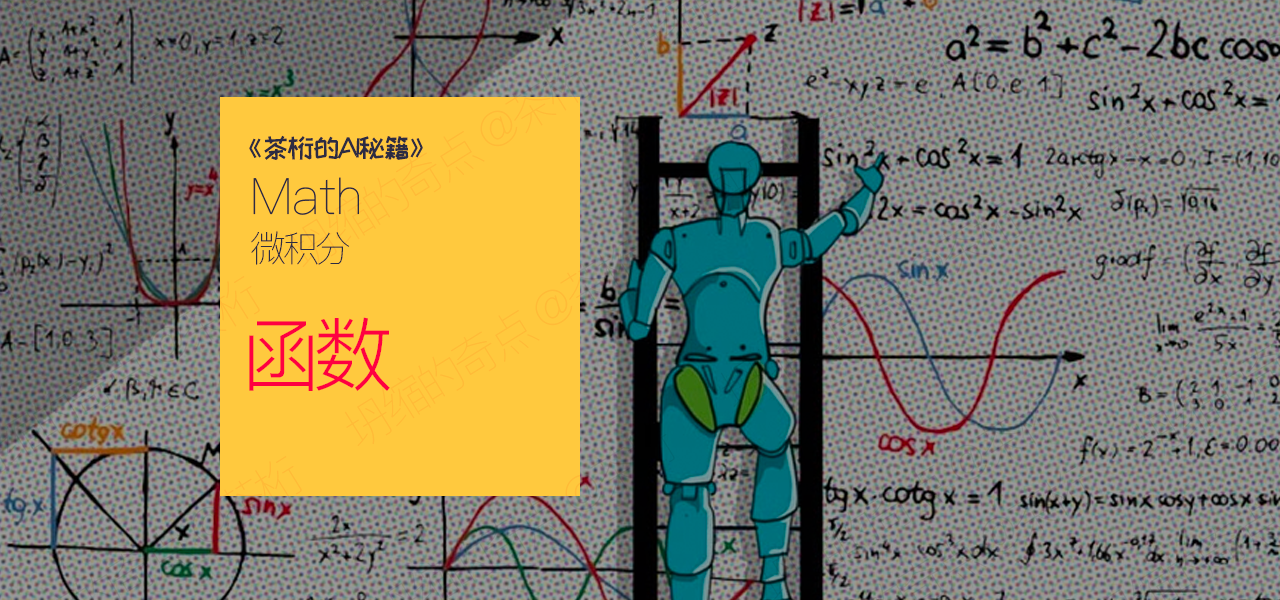
\includegraphics[width=1\textwidth]{asset/茶桁的AI秘籍_Math_6.png}
\end{figure}

\newpage

经历了前面5节课的基础之后, 不知道大家感觉怎么样?我后台接收到了一些反馈, 有的同学说比较简单; 有的同学说正合适; 有的同学就觉得有些绕, 一时之间可能没办法理解和接受. 说明同学们的水平还是有一些参差不齐的. 

其实每个人的背景都是很不一样的, 大家的方向也各有不同. 有CV方向, 有NLP的, 还有Data Science的. 可是也有很大一部分小伙伴也许就是零基础想要进行转行, 进入赛道. 

可是我也只能写这么一份, 会尽量照顾到大部分人, 可能会针对初学者而言比较友好一点. 咱们不可能真把这几节课当成是数学系的同学专研的那种. 那么对于基础有些过分薄弱的, 希望同学们课下能多发挥一下自主学习的能力, 躲在其他地方进行一下补足. 咱们这节数学课虽然比较偏基础, 但也并不可能一点难度没有. 所以基础太过薄弱的同学, 课下稍微去努努力, 夯实一下自己的数学底子. 

咱们AI秘籍的课程, 以后也会有很多时候是需要自己去不断练习, 发现问题解决问题. 那同学们必须学会自己去自主学习. 咱们的课程就只是将最主要的知识点讲给大家, 带大家一程. 更重要的是你要学会如何自己解决问题. 有问题的, 可以后台留言问我, 但是你指望我手把手带那就有点不太现实了. 如果你之后进入了这一行, 或者说不管你做哪一行, 工作的时候指望着有一个人手把手的教你那肯定是不可能的对吧?领导看到你这样的话肯定很生气, 到了年底的时候也许给你末位淘汰. 所以还是希望大家自己能发现问题, 并且自己知道如何去解决问题. 

好了, 话不多说, 我们开始今天的课程. 今天开始, 之后的几节课都是关于\textit{微积分}. 

微积分是我们在数学领域很重要的一个部分, 我们在之前的基础部分里面已经说过AI方面\hyperlink{数学如何运用于AI}{需要哪一些数学知识}, 第一个就是微积分. 当然其他还有线性代数、概率统计、图论这些. 

\hypertarget{6.微积分-函数}{}
\section{函数}

我们开始的第一个内容, 就是函数. 在基础课里面说过, 函数是有很多种不同样的形状的. 可以是一元, 也可以是多元的. 就比如说一次函数、二次函数、正旋、以及指数函数、对数函数. 

\begin{align*}
  & y = x + 1 & y = x^2 \\
  & y = sinx & y = e^x \\  
  & y = log_2^x & z = x^2 + y^2 \\ 
  & ...
\end{align*}

函数包括的种类其实非常多, 化成的函数图像也是非常的多样性. 各个函数对应的函数关系不一样. 比如图\ref{fig:img7_1}右下角的那个图形, 就是二元函数的图像. 其中X、Y是作为自变量, Z是在XY的基础之上去构建的一个三维的图形. 

\begin{figure}[ht]
  \centering
  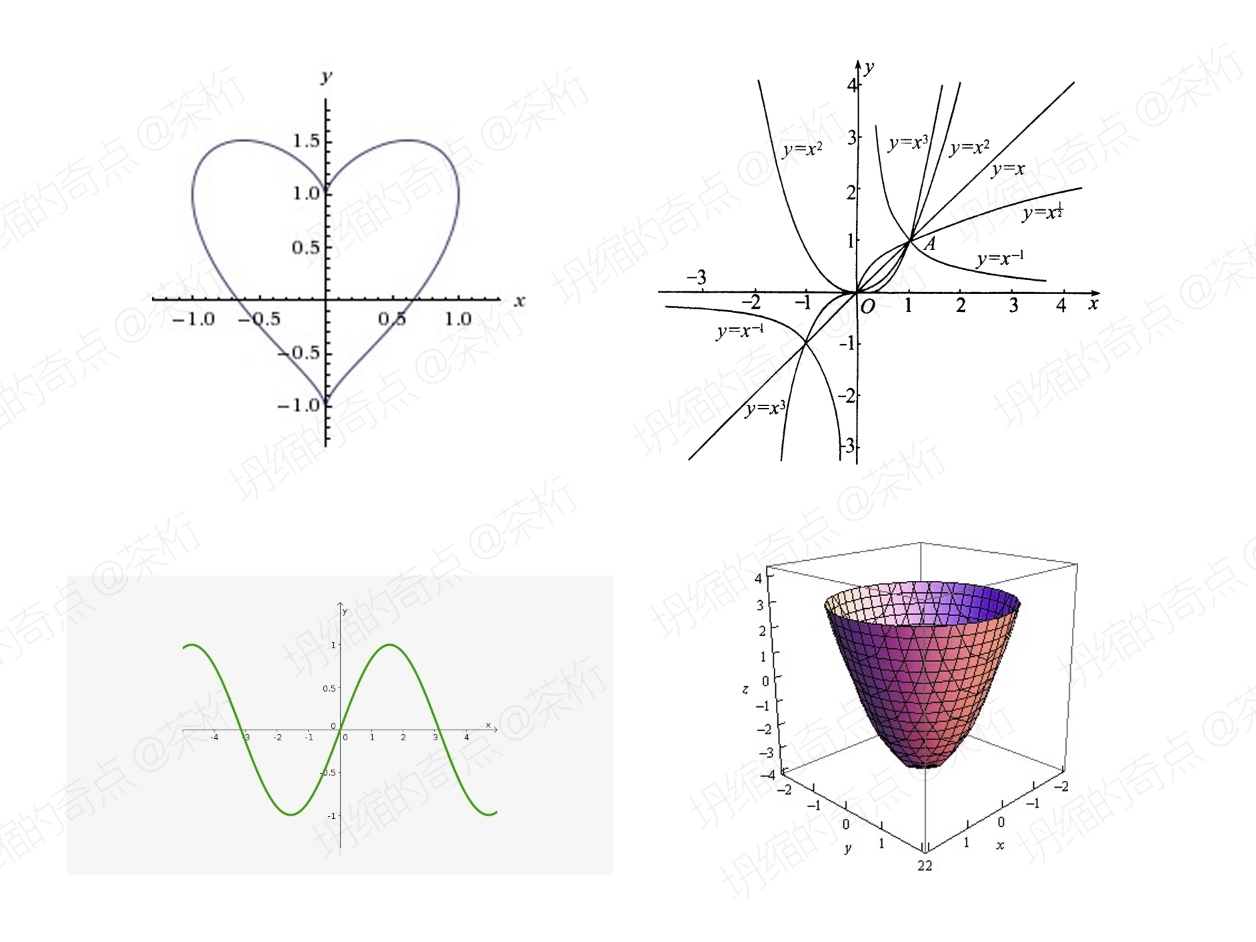
\includegraphics[width=1\textwidth]{asset/0c36f8c5-0b4f-4fc1-a5dc-a206fd7e2db2.png}
  \caption{不同的函数图形}
  \label{fig:img7_1}
\end{figure}

看了之前课程的小伙伴应该还记得, 左上角的那个图像其实它不是函数的图像. 因为它一个X对应的两个Y值, 

从本质上面来说, 如果我们抽象一点, 函数它其实是从一个集合到另外一个集合的一种映射规则: $f:R -> R$.

这么说可能会有点抽象, 集合和映射规则什么意思?这里的集合就和我们日常生活当中理解的集合差不多. 就是一堆东西, 然后把它们聚在一起形成的一个聚合体, 我们把它叫做集合. 

在数学上面的集合可以理解为一个数的集合, 数的一个聚合体. 

所以函数其实就是给你一个集合, 然后再给你一个映射规则. 规则可以把集合里面的每一个数给映射到另外一个集合里面. 

就是在映射规则之下, 右边的集合里面有一个数会和左边里面的数一一对应. 

R在数学上表示实数集. 实数、虚数、负数大家应该有听过吧?即便没学过的同学应该有听过. 实数就是我们在自然界当中可以接触到的实际存在的这些数字, 比如说你的身高多少, 世界上有多少个国家, 这些东西都是有实际意义的. 

虚数是什么呢?比如-1的平方根 $\sqrt{-1}$, 按照实数的理解来说它是不存在的. 那任何数的平方就是自己乘自己, 它肯定是一个非负数, 怎么可能是-1呢?但是在数学上面它确实存在, 我们在现实生活当中可能不太会遇到. 

函数之前讲过, 是从一个集合到另外一个集合的一种映射规则. 就像是你把你的手放在蜡烛前面, 蜡烛就会通过光把你手形成的影子投在墙壁上. 那手和墙上的影子就是类似于这么一种映射规则. 

函数可以是很天然的, 比如:

\begin{align*}
  y & = e^x; \\
  y & = sinx;
\end{align*}

这两个式子中, 咱们先来看$y=e^x$, e叫自然对数, 就有点像是生物物种不受任何限制的去增长, 它的种群数量会是一个爆炸式的增长. 就可以用$y=e^x$来表示. 

$y=sinx$, 是正弦. 在发电站里面发的交流电就是这种正弦波的形式, 也是来自于自然的. 

当然也可以人工去创造一些函数. 比如迪利克雷函数非常有意思. 当X是有理数的时候, 函数值是1, X是无理数, 函数值是0. 

看到这里先停下思考下, 你觉得迪利克雷函数的图像应该长成什么样子? 我在这里做了一个刻意的排版,将图放在了下一页。大家先畅想一下, 不要急着往下看, 给自己一点时间想想, 按照这种规则, 吉利克雷函数的图像应该长成什么样?

\begin{align*}
  f(x) = 
  \begin{cases}
    1, \qquad  x \mbox{是有理数} \\
    0, \qquad  x \mbox{是无理数}
  \end{cases}
\end{align*}

如果在不考虑到精确度的情况下, 我们可以把它的函数图像画成图\ref{fig:img7_2}的样子. 

我们来看, 上下各有一条平行线对吧?肉眼看上去上下是一条平行线, 但其实图像只是看似连续的, 实际上这些线并不是连续的, 是无限多个点. 

\begin{figure}[ht]
  \centering
  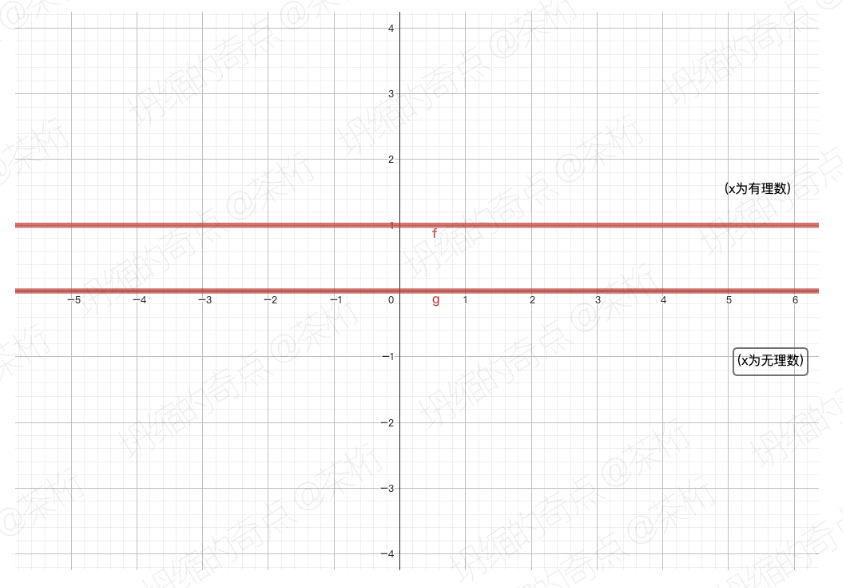
\includegraphics[width=0.8\textwidth]{asset/97060faa-bcf8-4fdb-8f69-e42425ab9575.png}
  \caption{迪利克雷函数的图像}
  \label{fig:img7_2}
\end{figure}

因为实数有个稠密性, 就是说有理数也是无限多的, 无理数也是无限多的. 在任意小的一个区间之内, 他俩都是无限多的, 那些断点你肉眼看不着. 所以, 其实\textbf{迪利克雷函数虽然是客观存在的, 但是我们无法画出来}. 上面图像只是一个近似. 

现在我们知道, 函数抽象来说是一个什么样的东西: 是一种映射的法则. 那我们应该怎么样去表示它呢?

首先很熟悉的, 我们知道可以用解析式去表示. 一个自变量X、一个因变量Y, 他们之间的一种数量关系. 

解析式: \(y = e^x\)

还有可以通过文字描述的形式, 就像迪丽克雷函数: \textit{自变量为无理数时因变量取值0, 有理数时取值1}. 一般都是通过这种方式去描述它. 

然后还有一种, 叫做列表法. 列表法就是把自变量值和应变量的值给它一一对应起来, 也可以代表一种映射规则. 

\begin{table}[ht]
  \centering
  \begin{tabular}{llllll}
    \midrule
      x & 1 & 2 & 3 & 4 & ... \\
      y & 2 & 4 & 6 & 8 & ... \\
    \bottomrule
  \end{tabular}
  \caption{列表法}
  \label{tab:table7_1}
\end{table}

结合刚才所说的这些内容总结一下, 函数主要包含三个部分:

\begin{itemize}
  \item 一个是定义域(整数域, 实数域, 复数域...)
  \item 一个值域(整数域, 实数域, 复数域...)
  \item 还有个映射法则(将定义域映射到值域)
\end{itemize}

映射法则就是作用在定义域上面, 把定义域里面的数给映射到值域上面. 结合我们手投影在墙上的例子来看, 把手比作定义域, 蜡烛可以看作映射法则. 蜡烛的光照在定义域上面, 就形成了墙上的影子, 就是值域. 

但是, 不是所有的映射法则都可以构成函数. 对于函数有一个比较严格的要求, 就是一个自变量在值域当中有且只能有一个因变量与它相对应. 如图 \ref{fig:img7_3}:

\begin{figure}[ht]
  \centering
  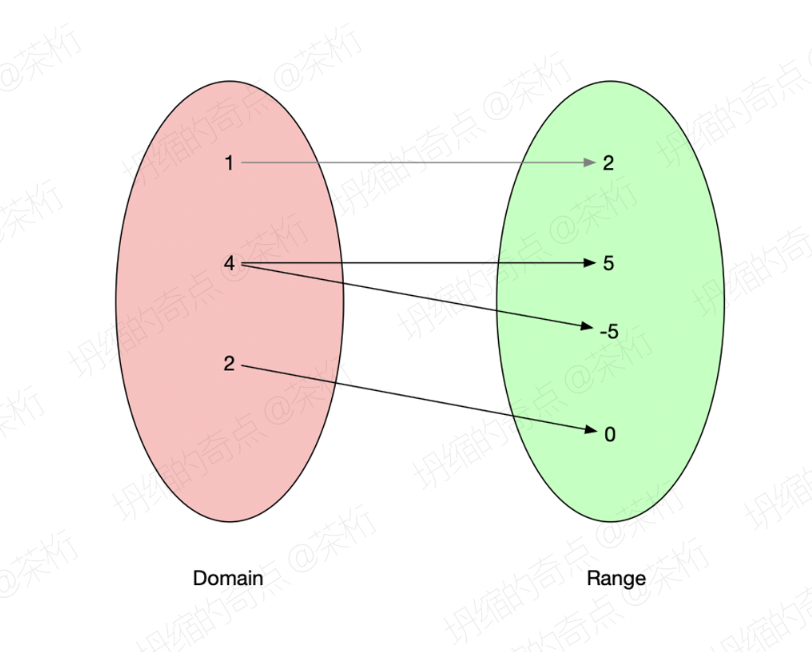
\includegraphics[width=0.55\textwidth]{asset/78b109d0-c39f-446b-ba0a-2b983138d76f.png}
  \caption{}
  \label{fig:img7_3}
\end{figure}

途中左边集合是定义域, 就是我们的手; 右边的集合就是墙上的影子. 我们会发现在映射规则之下, 数字4被映射到了值域里面的两个值上面. 是不可能的, 就像光照到你大拇指, 投在墙上只可能形成一个大拇指的影子, 不可能同时显出两个大拇指的影子. 除非有两个映射规则, 也就是有两个蜡烛. 所以这种映射规则就不能称作为函数. 

对于函数这部分的理解, 也差不多就讲到这里了. 大家只要把握住它是一种映射规则. 其实说白了就是一种转换规则. 然后, 它是作用于定义域的, 定义域的数在映射法则或者说转换法则的作用下映射到了值域上, 就是做了一种转换. 